\begin{frame}[fragile]
\frametitle{LA-CoNGA somos un consorcio}

\begin{tikzpicture}[node distance=1.25cm, auto,]
 %nodes
 \node[inner sep=0pt] (mapa) at (7.2,-3.2)
    {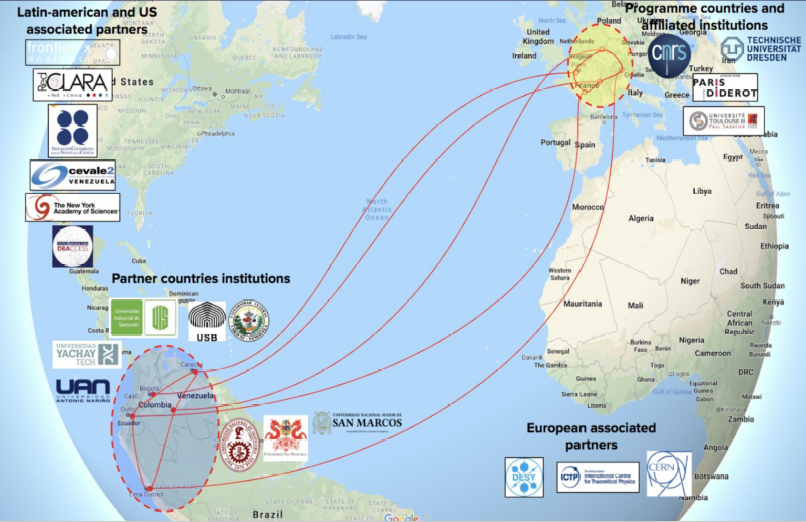
\includegraphics[scale=0.35]{imagenes/mapaColab.png}};
 \node[socio] (academic) at (0,-0.9) {{\small Socios Académicos}};
 \node[below=of academic] (dummy1) {};
 \node[socio, right=of dummy1] (industrial) {\small Socios Industriales}
 	edge[pil,<->,bend right=45] (academic.east);
 \node[below=of dummy1] (dummy2) {};
 \node[below=of dummy2] (dummy) {};
 \node[socio,left=of dummy2] (cientific){\small Socios Científicos}
 	edge[pil,<->,bend left=45] (academic.west)
 	edge[pil,<->,bend right=45] (industrial.south);
 \node[right=of industrial] (dummy3) {};
 \node[right=of dummy3] (dummy4) {};
 %\node[resumen, below=of dummy3] (resumen) {{\bf\color{LCredInst} Resumen}\begin{itemize}
 \node[resumen] (resumen) at (1.5,-5.8) {\small \begin{itemize}
 \item[-] Universidades (11)
 \item[-] Socios científicos e industriales (13)
 \item[-] Total: 24 instituciones.
 \end{itemize}};
 
 \end{tikzpicture}

\end{frame}

\begin{frame}[fragile]
\frametitle{LA-CoNGA somos: Universidades socias LA}
\begin{columns}[c] % The "c" option specifies centered vertical alignment while the "t" option is used for top vertical alignment

\column{.58\textwidth}
\begin{itemize}
	\item Colombia:
	\begin{itemize}
		\item Universidad Antonio Nariño (UAN)
		\item Universidad Industrial de Santander
(UIS) {\bf (coordinadora LA)}.
		\end{itemize}
	\item Ecuador:
	\begin{itemize}
		\item Universidad San Francisco de Quito
(USFQ).
		\item Universidad Yachay Tech (UYT).
		\end{itemize}
	\item Perú:
	\begin{itemize}
		\item Universidad Nacional de Ingeniería
(UNI).
		\item Universidad Nacional Mayor de San
Marcos (UNMSM).
		\end{itemize}
	\item Venezuela:
	\begin{itemize}
		\item Universidad Central de Venezuela
(UCV).
		\item Universidad Simón Bolívar (USB).
		\end{itemize}
\end{itemize}


\column{.38\textwidth} % Right column and width
\begin{center}
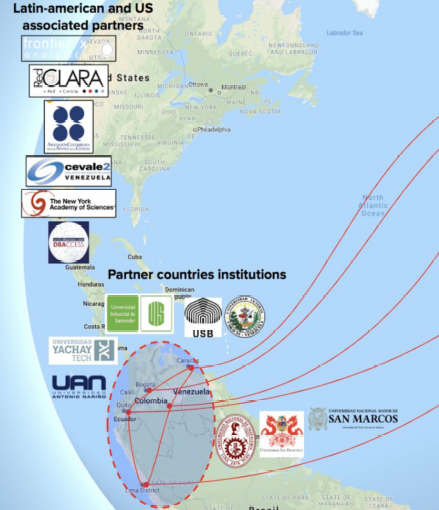
\includegraphics[scale=0.5]{imagenes/mapaColab_1.png}
\end{center}

\end{columns}
\end{frame}


\begin{frame}[fragile]
\frametitle{LA-CoNGA somos: Universidades socias UE}
\begin{columns}[c] % The "c" option specifies centered vertical alignment while the "t" option is used for top vertical alignment

\column{.58\textwidth}
\begin{itemize}
	\item Alemania:
	\begin{itemize}
		\item Technische Universitat Dresden (TUD).
		\end{itemize}
	\item Francia:
	\begin{itemize}
		\item Universitè de Paris (UdP) {\bf (líder)}
		\item Universitè Touluse III Paul Sabatier (UPS)
		\end{itemize}
\end{itemize}

\column{.38\textwidth} % Right column and width
\begin{center}
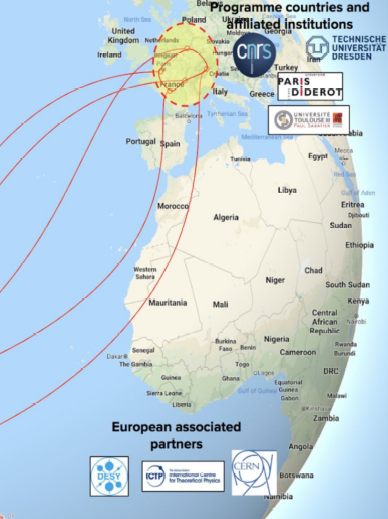
\includegraphics[scale=0.5]{imagenes/mapaColab_2.png}
\end{center}

\end{columns}
\end{frame}

\note{sociosCienInd}

\begin{frame}[fragile]
\frametitle{LA-CoNGA somos: Socios Científicos e Industriales}

\begin{center}

\includegraphics[scale=0.5]{imagenes/sociosCienInd.png}
\end{center}

\end{frame}

\begin{frame}[fragile]
\frametitle{LA-CoNGA somos: La gente NS 2021}

\begin{center}
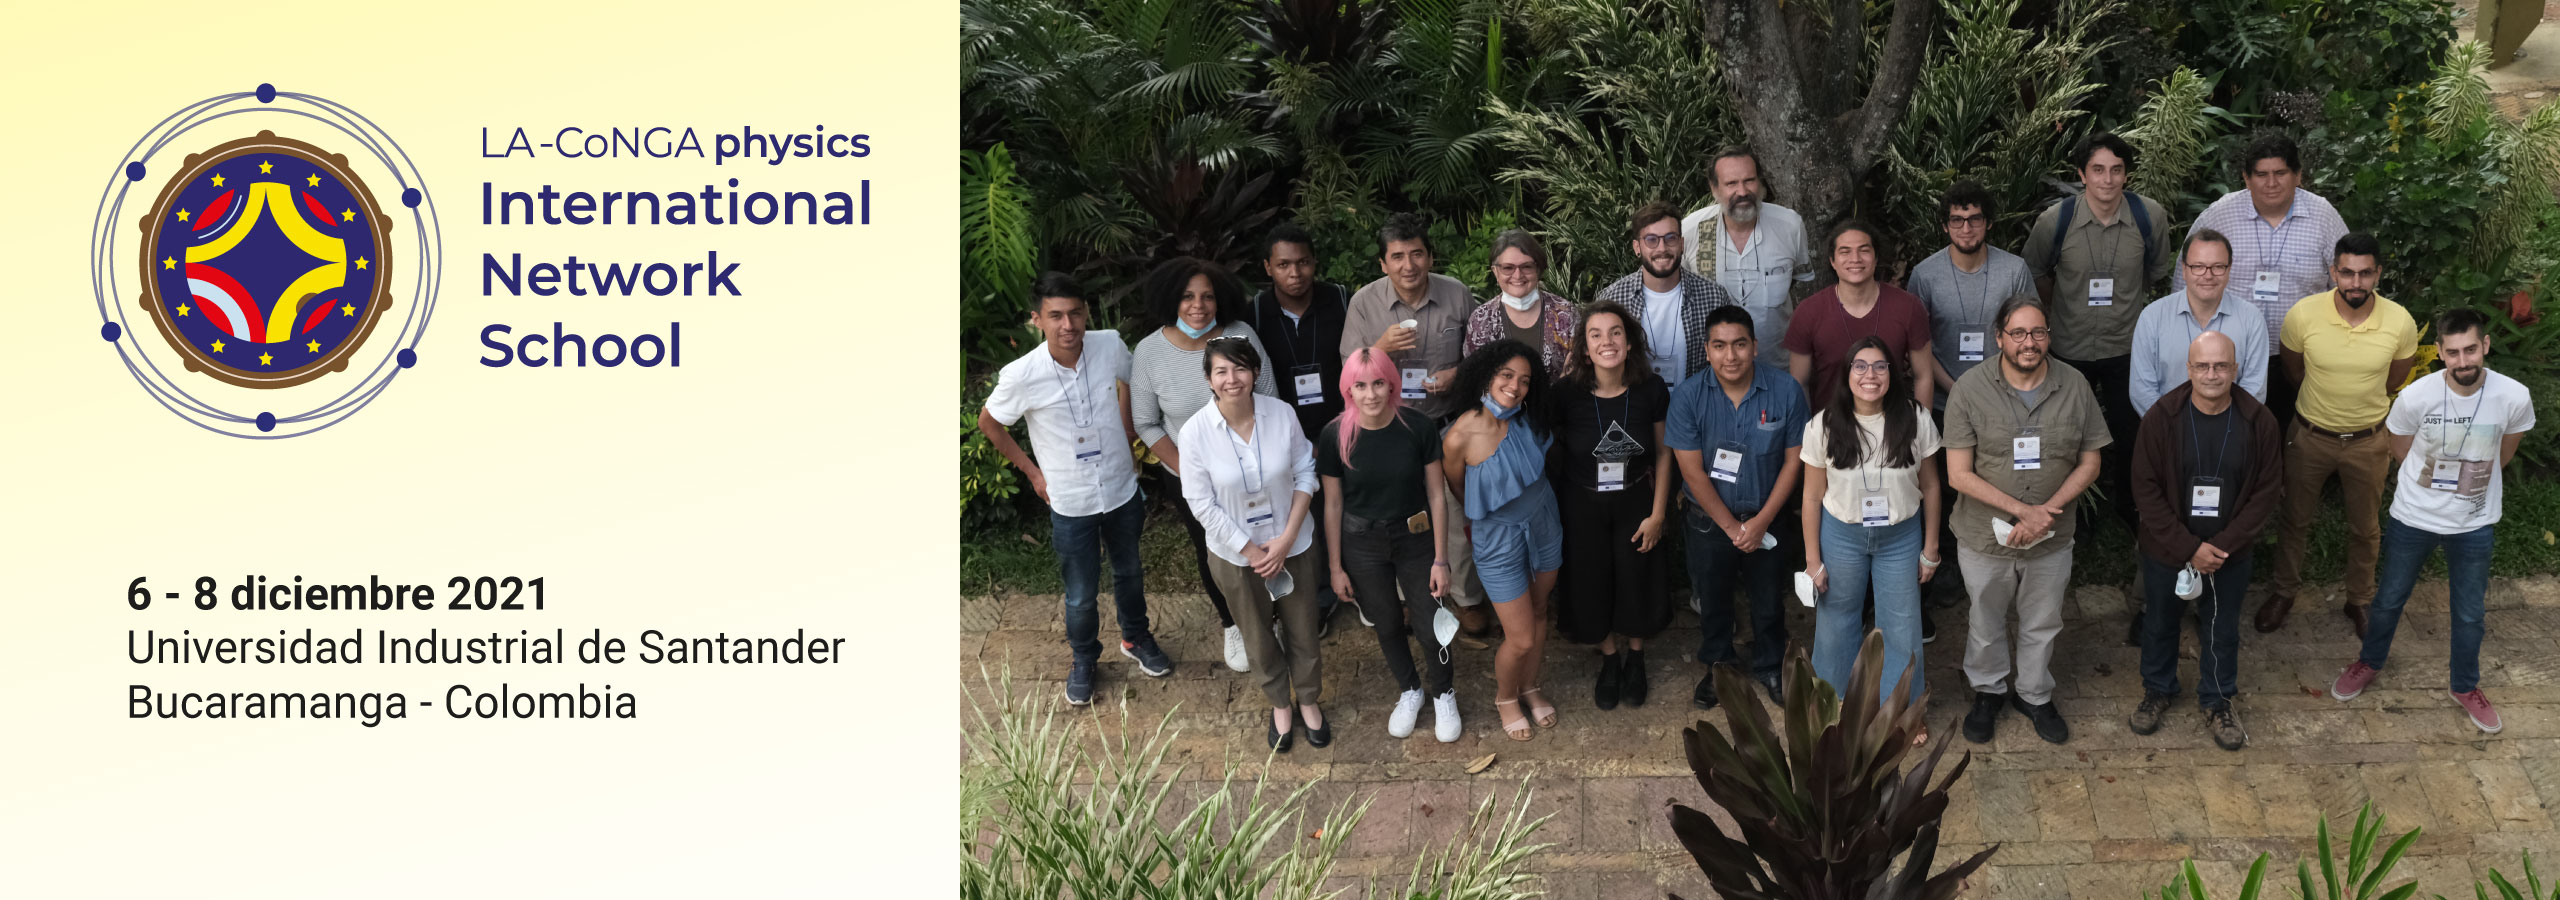
\includegraphics[scale=0.15]{imagenes/banner-2021-bucaramanga.jpg}
\end{center}

\end{frame}

\begin{frame}[fragile]
\frametitle{LA-CoNGA somos: La gente NS 2022}

\begin{center}
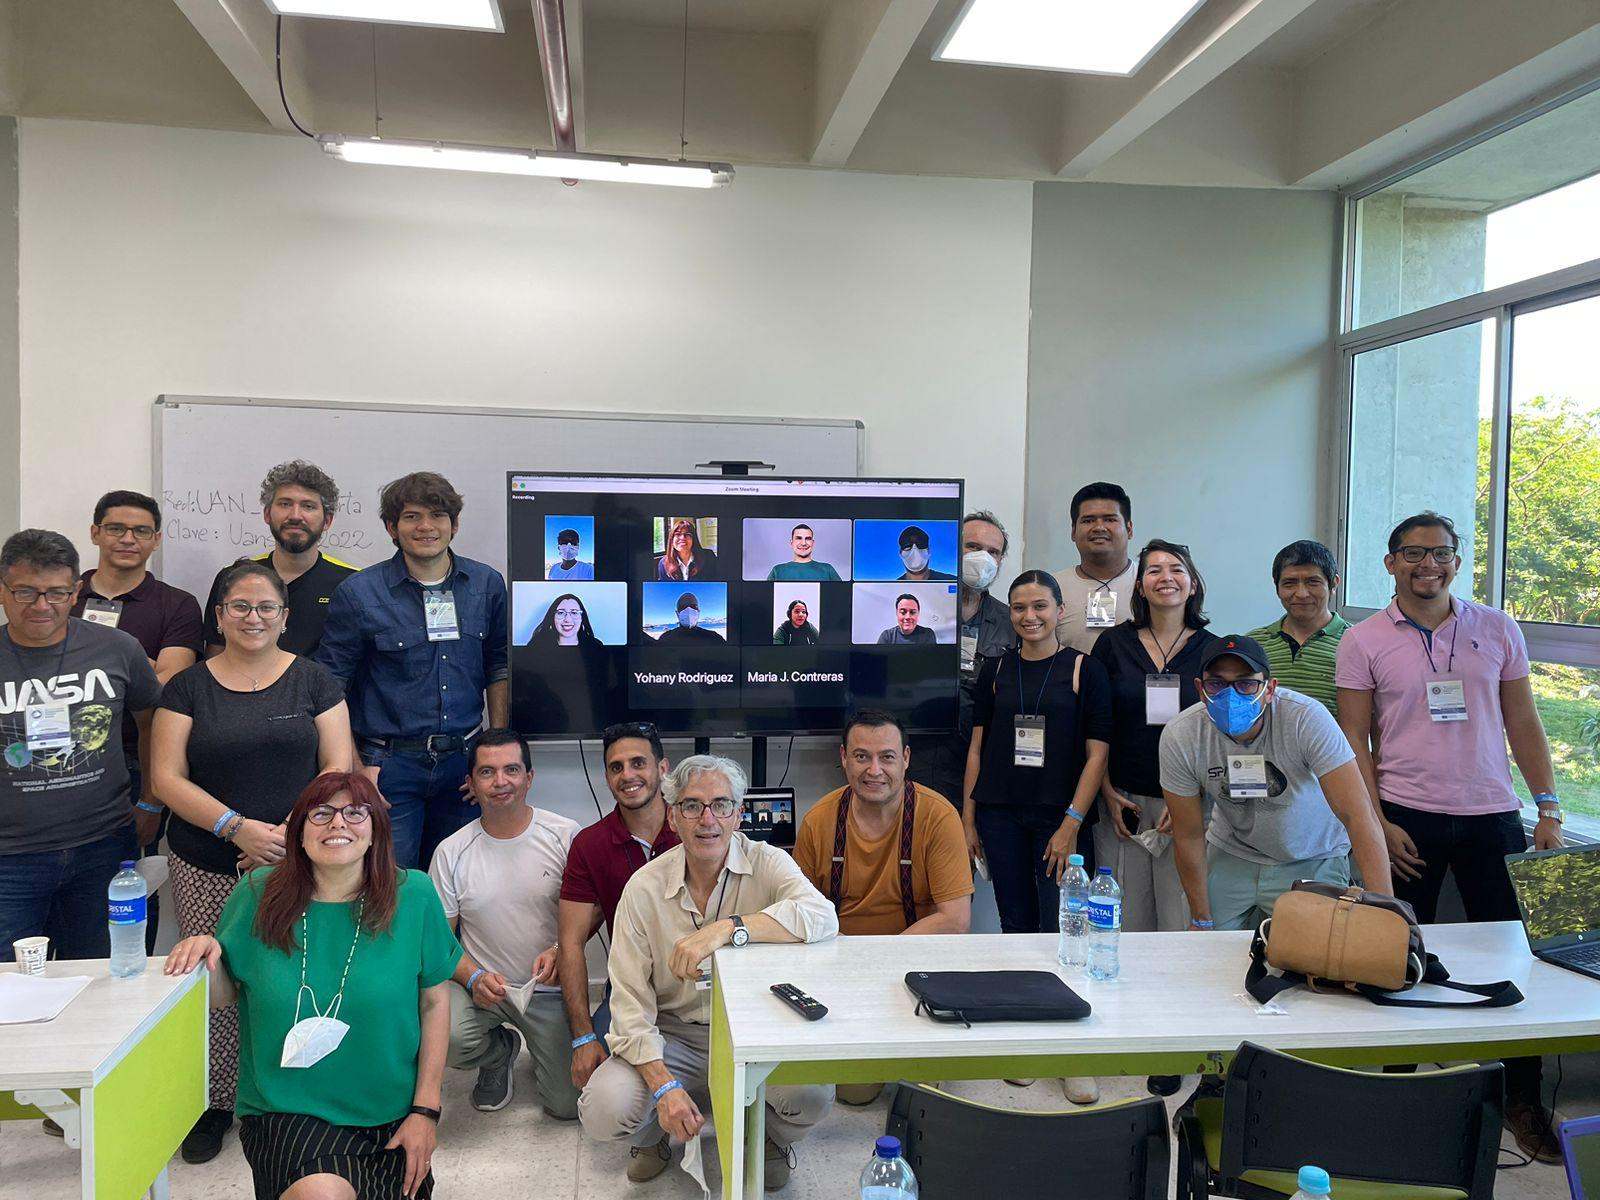
\includegraphics[scale=0.15]{imagenes/grupoNS2022.jpg}
\end{center}

\end{frame}

